% -*- TeX -*- -*- UK -*- -*- Soft -*-"

\chapter{Setting up WinEdt}

\section{Install WinEdt}
\label{sec:installwinedt}
This document assumes that WinEdt v.10.0 is installed.

After you changed an ini file, the changes can be immediately be made available by clicking on the load button:

\centerline{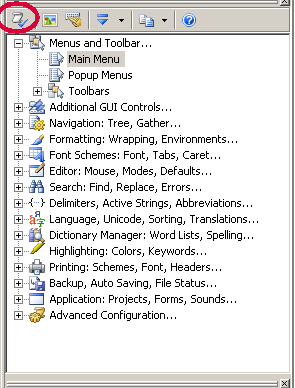
\includegraphics[bb= 0 0 295 388, width=0.4\textwidth]{eps/loadini.png}}

After you make changes to a particular script you should use the Load Command (the first button in the Option Interface Toolbar) to make the changes effective immediately. It is not necessary to restart WinEdt. In fact, no scripts are loaded at startup: the compiled raw data is stored in WinEdt.dnt (Do Not Touch). This reduces the startup time and reduces the likelihood of error messages during startup.


I am not quite sure how to activate the changes for the next time you start WinEdt.  It seems that exporting to WinEdt.dnt have the effect of saving the changes to that these are working next time you load WinEdt.

\begin{lstlisting}

\section{Viewer Setup}

Yap seemed to fail on my WinEdt install.

MikTeX provides a DVI viewer, called YAP that integrates well with WinEdt. If properly set up, WinEdt and YAP are synchronised. When you run the \LaTeX{} compiler, YAP will open at the location of the cursor in the WinEdt file. When you double click in the YAP window, the text cursor in WinEdt will move to the corresponding location.

The Yap binary is located in the MikTeX bin file, on my PC at
\url{C:\Program Files\MiKTeX 2.9\miktex\bin\x64}

$<$Options$>$$<$Execution Modes$>$, select 'LaTeX'. If not set, set 'Wait for execution to finish' and select the 'Start Viewer' and 'Forward Search' boxes. The 'Start Viewer' selection will start the viewer after completion of the compilation process, and the 'Forward Search' selection will move a small, round, cursor to the location in the DVI viewer, where the cursor is in the LaTeX document (when it makes sense).

Other viewers can be started in a similar manner, just select the appropriate compiler in the left-hand box, and set 'Start Viewer' in the next box.


\centerline{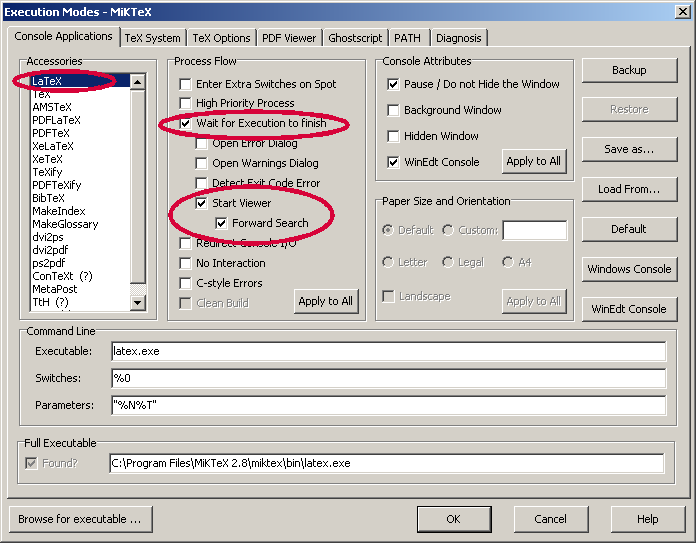
\includegraphics[bb= 0 0 696 543, width=\textwidth]{eps/StartViewer.png}}

In YAP go to  $<$View$>$$<$Options$>$$<$Inverse Search$>$, select WinEdt, if not yet selected. If option 'WInEdt' does not show in the dropdown box,  you have to enter the path to the application in the text box at the bottom of the dialog box.  On my installation, the entry is	\\
{\small \verb+"C:\Program Files\WinEdt Team\WinEdt 10\winedt.exe" "[Open(|%f|);SelPar(%l,8)]"+}

\centerline{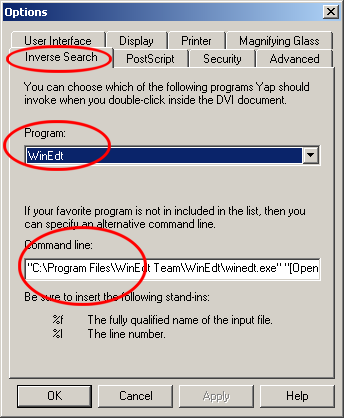
\includegraphics[bb= 0 0 344 416, width=.6\textwidth]{eps/yapinverse.png}}


\section{Enabling Active Strings for  begin-end Pair}
It seems that the default settings are acceptable, no edit required. If you do need to change anything, go to
$<$Options$>$$<$Options Interface$>$$<$Delimiters, Active Strings, ...$>$$<$Active Strings$>$, edit the macro file just opened. Edit as required and save when done.

\centerline{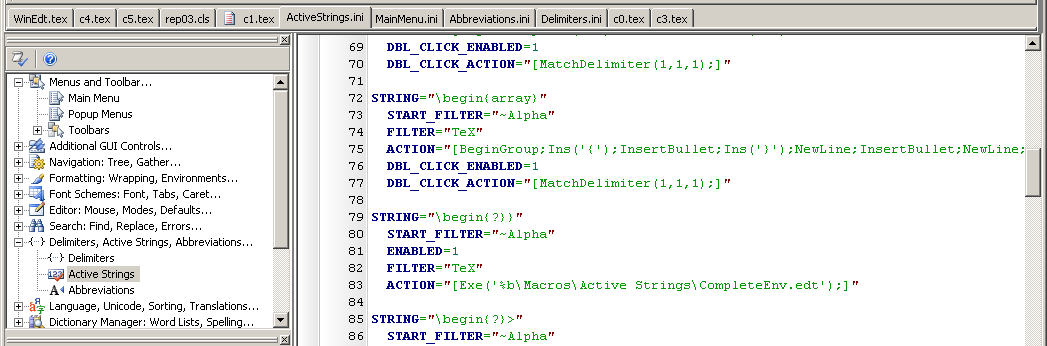
\includegraphics[bb= 0 0 1047 346, width=\textwidth]{eps/ASbegin.png}}

%It seems in WinEdt9, that you must type \verb"\begin{enumerate}}", i.e. with an extra \verb"}" to %activate the active string.


\section{Setting up the Dictionary}
$<$Options$>$$<$Options Interface$>$$<$Dictionary Manager:....$>$$<$Word Lists (.)...$>$, edit the macro file just opened.  You enable or disable
sub-dictionaries according to your requirement.

If you require only UK English, as in in South Africa, select:\\
\textbf{Enable the following dictionaries:} User (Addon), EDT, LaTeX, WinEdt, English (common),  English (colour),  English (labelled),  English (centre), English (ise),  English  (yse).\\
\textbf{Disable the following dictionaries:}  English (Small), English (color), English (labeled), English (center), English (ize), English (yze). 
Save the file when done.

\centerline{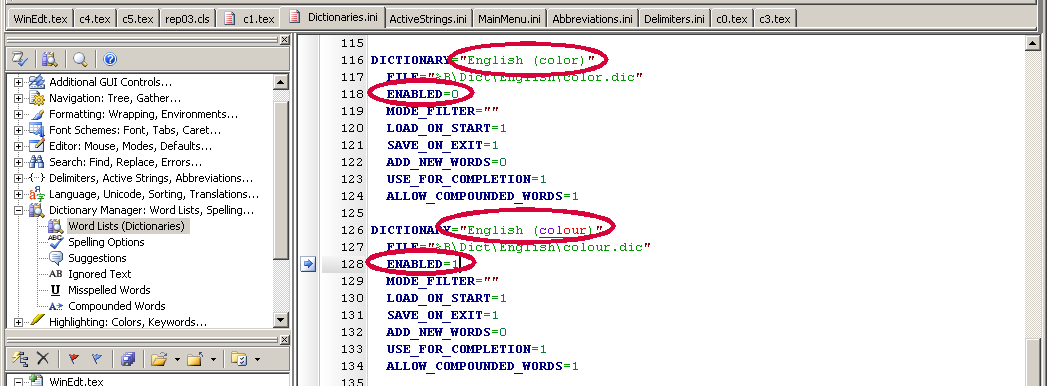
\includegraphics[bb= 0 0 1047 386, width=\textwidth]{eps/dictionary.png}}

If you want both the UK and US English dictionaries, keep all of the above dictionaries on. You can then select the language on a per-file basis.
Use embedded emacs-style mode and submode commands as the first line of each file. For example, use\\
\verb"% -*- TeX -*- -*- US -*- -*- Soft -*-" for US spelling, or\\
\verb"% -*- TeX -*- -*- UK -*- -*- Soft -*-" for UK spelling in the tex file.\\
For more information search the WinEdt documentation for ``modes and submodes''.\\
See also
\begin{lstlisting}
\url{https://www.gnu.org/software/emacs/manual/html_node/emacs/Specifying-File-Variables.html}
\url{https://www.gnu.org/software/emacs/manual/html_node/emacs/Choosing-Modes.html}
\end{lstlisting}


\section{TeX Symbols GUI}

Activate the TeX Symbols GUI by clicking on the $\Sigma$-on-the grid symbol.

\centerline{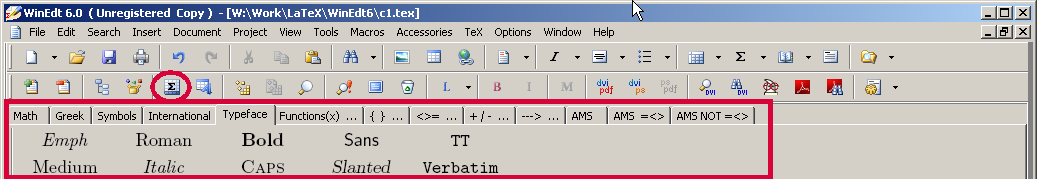
\includegraphics[bb= 0 0 1037 179,width=\textwidth]{eps/texsymbolsgiu.png}}



\section{Keep Whitespace at EOF and EOL}

$<$Options$>$$<$Options Interface$>$$<$Editor: Mouse, Modes,...$>$$<$Defaults$>$, edit the macro file just opened. Scroll down to 'Trim Spaces' and 'Trim lines' and disable these two --- this is stop WinEdt from removing spaces at the end of lines and files.

\centerline{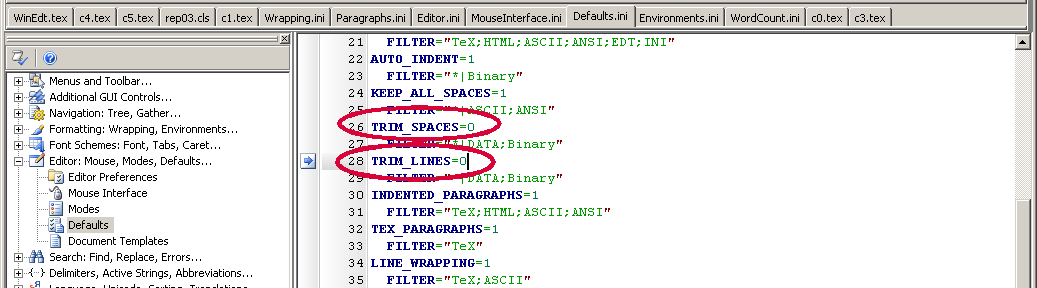
\includegraphics[bb= 0 0 1037 288,width=\textwidth]{eps/trimeoleof.png}}


\section{Set Text Wrapping and Text Width}

$<$Options$>$$<$Options Interface$>$$<$Formatting, Wrapping, Environments....$>$$<$Wrapping$>$, edit the macro file just opened.

\centerline{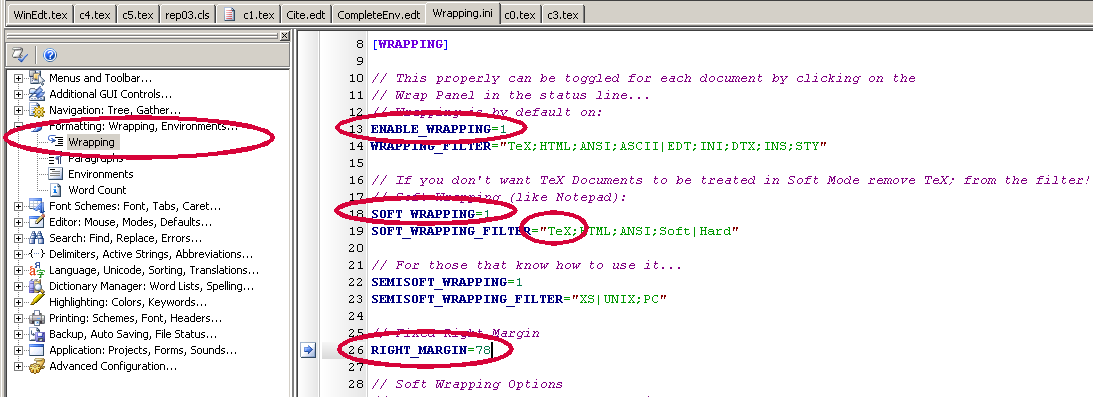
\includegraphics[bb= 0 0 1093 397,width=\textwidth]{eps/wrapping.png}}

\section{Add a Table-Paste Macro to a Menu}
\label{sec:addpastetable}

$<$Options$>$$<$Options Interface$>$$<$Menus and Toolbar$>$$<$Main Menu$>$, edit the macro file just opened. Add the text shown below at the indicated location.

\centerline{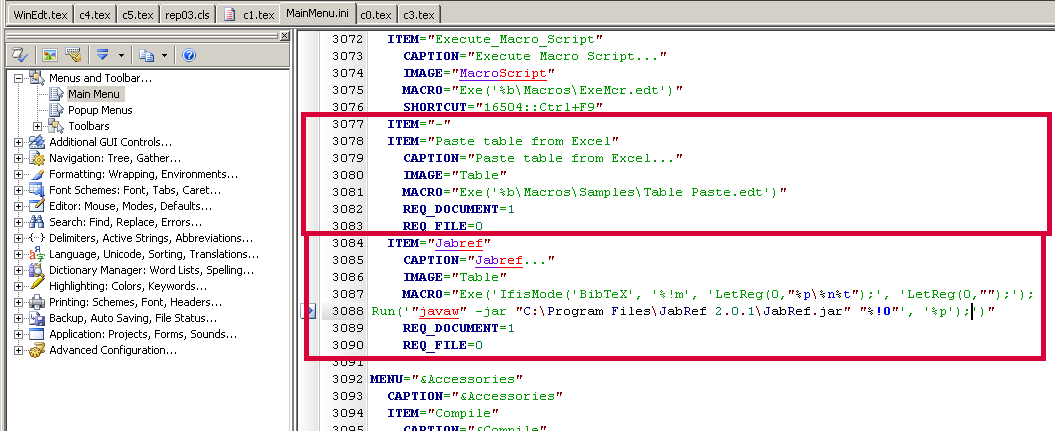
\includegraphics[bb= 0 0 1055 431,width=\textwidth]{eps/AddExcelTable.png}}


The picture above shows intalling JabRef, this is optional if installed.

\begin{lstlisting}[label=MacropastetableExcel,caption=Macro to paste table from Excel]
    ITEM="Paste table from Excel"
    CAPTION="Paste table from Excel..."
    IMAGE="Table"
    MACRO="Exe('%b\Macros\Samples\Table Paste.edt')"
    REQ_DOCUMENT=1
    REQ_FILE=0
\end{lstlisting}
just before the \lstinline{END="&Macros"} line.


Copy and paste the text in Listing~\ref{MacropastetableExcel}. If it does not work,  check the MACRO line:  take care to use the upquote (\verb+'+,  next to the Enter key) and not the curly quote (').
Then copy the following file (\lstinline{Table Paste.edt}) from the repo to the 
\lstinline{C:/Program Files/WinEdt Team/WinEdt 10/Macros/Samples}.
folder.

\begin{lstlisting}
    // %-*- ASCII -*- -*- EDT -*-
    //
    // Paste Table and covert it to LaTeX format:
    //  Tab  -> &Tab
    //  EOLN -> \\EOLN

      Requires(20010317);  // Requires WinEdt 5 Build 20010317 (or later)

      CopyFromClipboard(0);  // Get the Clipboard Text Data (eg. Excel)

      // Convert Tab to &Tab
      LetRegNum(2, -2);
      Loop(!|>
        FindInString("%!0", "$[#9]$", 1,2, 1011, %!2+2);>
        IfOK(!'ReplaceInString("%!0", "&\&9;", %!1, %!2, 1, 0);',!'Stop;')|);

      // Convert EOLN to \\EOLN
      LetRegNum(2, -3);
      Loop(!|>
        FindInString("%!0", ">", 1,2, 1011, %!2+3);>
        IfOK(!'ReplaceInString("%!0", "\\\\>", %!1, %!2, 1, 0);',!'Stop;')|);

      InsText("%!0"); // Insert with no wrapping

    End;

    // WinEdt also has a Block/ Column mode selection that can come
    // handy when manipulating aligned tables...
\end{lstlisting}




\section{Add a Back Slash to Forward Slash Macro to a Menu}
\label{sec:bsfs}

$<$Options$>$$<$Options Interface$>$$<$Menus and Toolbar$>$

Search down for the entry labelled \lstinline{MENU="&Accessories"}.
In the section just before Accessories, add the following:
\begin{lstlisting}
    ITEM="Backslash to Forward"
    CAPTION="Backslash to Forward..."
    IMAGE="Table"
    MACRO="Exe('%b\Macros\Samples\bstofs.edt')"
    REQ_DOCUMENT=1
    REQ_FILE=0
\end{lstlisting}
just before the \lstinline{END="&Macros"} line.

Add the file (\lstinline{bstofs.edt}) with the following contents to
\lstinline{C:/Program Files/WinEdt Team/WinEdt 10/Macros/Samples/bstofs.edt} 

\begin{lstlisting}
SetFindStr("\");
SetReplaceStr("/");
SetSearchCaseSensitive(0);
SetSearchRelaxed(0);
SetSearchWholeWords(0);
SetSearchInline(0);
SetRegEx(0);
SetSearchSelected;
SetSearchCyclic(0);
SetSearchForward(1);
SetSearchEntire(0);
SetReplaceRespectCaps(1);
SetReplacePrompt(0);
SearchReset;
ReplaceAll;
// ReplaceDialog;
\end{lstlisting}


\section{Disable Synctex}

In WinEdt10 the default settings for LaTeX is to compile with option -synctex=-1 and, in WinEdt5.6, the default settings for LaTeX is without the -synctex option.
However, MiKTeX does not support the synctex option for filenames with spaces.

The solution is to open WinEdt and uncheck 'Use -synctex switch' in $<$Options$>$ $<$Execution Modes$>$$<$PDF Viewer$>$.

\centerline{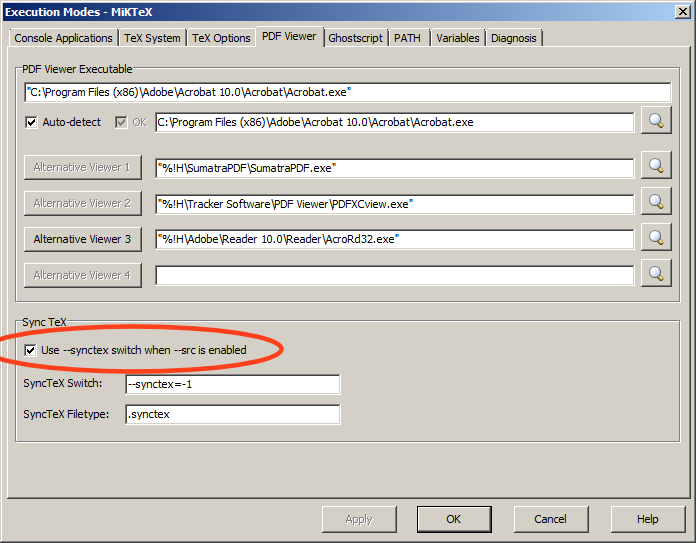
\includegraphics[bb= 0 0 696 543,width=0.8\textwidth]{eps/synctex.png}}

In the latest installs on Windows 7 it seems that this is no longer required; there can be spaces now. Experiment and find the best solution.


\section{Disable Autosaving and Backup}

Disable auto-saving and keeping backup files, by $<$Options$>$ $<$Preferences$>$$<$Backup$>$ and unchecking the relevant boxes.

\centerline{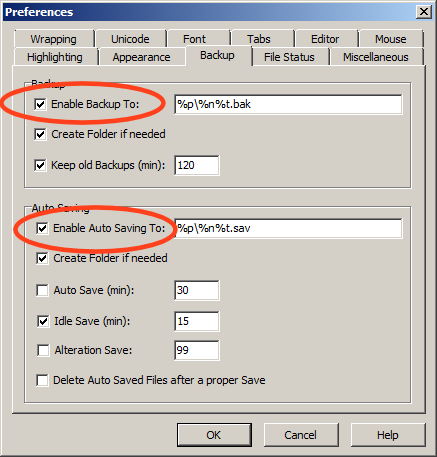
\includegraphics[bb= 0 0 437 457,width=0.6\textwidth]{pic/savingback.png}}




\section{Adding to TeX Symbols }
You may want to add new buttons to the \TeX\ symbols Typeface GUI such as adding new buttons to \url{Typeface.bmp} found in \url{C:\Program Files\WinEdt Team\WinEdt 10\Bitmaps\Gui}.  It may be necessary to copy the bitmap file to \url{C:\Program Files\WinEdt Team\WinEdt 10\Bitmaps\Gui125}. I am not quite sure what the different GUI folders are used for.

\centerline{
\includegraphics[bb= 0 0 999 88, width=\textwidth]{pic/Typeface.png}}

Add the new buttons to the current image, taking care that you keep the new buttons the same size.

$<$Options$>$$<$Options Interface$>$$<$Additional GUI Controls...$>$$<$TeX Symbols$>$, edit the macro file just opened. Locate this section corresponding to the Typeface part of the GUI and enter one of the following blocks.

\begin{lstlisting}
  PAGE="Typeface"
  CAPTION="Typeface"
  CONFIG_FILTER=""
  MODE_FILTER=""
  GROUP="Typeface.bmp"
    TOP=0
    SPACE=0
    ROWS=2
    COLUMNS=9
    WIDTH=111
    HEIGHT=32
    ITEM="\emph{...}"
      MACRO="Exe('%b\Macros\Fonts\Emphasize.edt');"
    ITEM="\textrm{...}"
      MACRO="Exe('%b\Macros\Fonts\Roman.edt');"
    ITEM="\textbf{...}"
      MACRO="Exe('%b\Macros\Fonts\Bold.edt');"
    ITEM="\textsf{...}"
      MACRO="Exe('%b\Macros\Fonts\SansSerif.edt');"
    ITEM="\texttt{...}"
      MACRO="Exe('%b\Macros\Fonts\TypeWriter.edt');"
    ITEM="\url{...}"
        MACRO="Exe('%b\Macros\Fonts\FormatURL.edt');"
    ITEM="\inline{...}"
        MACRO="Exe('%b\Macros\Fonts\FormatInline.edt');"
    ITEM="\index{...}"
        MACRO="Exe('%b\Macros\Fonts\FormatIndex.edt');"   
    ITEM="\textsup{...}"
        MACRO="Exe('%b\Macros\Fonts\Formattextsuperscript');"   
    ITEM="\textmd{...}"
      MACRO="Exe('%b\Macros\Fonts\Medium.edt');"
    ITEM="\textit{...}"
      MACRO="Exe('%b\Macros\Fonts\Italic.edt');"
    ITEM="\textsc{...}"
      MACRO="Exe('%b\Macros\Fonts\SmallCaps.edt');"
    ITEM="\textsl{...}"
      MACRO="Exe('%b\Macros\Fonts\Slanted.edt');"
    ITEM="\verb""..."""
      MACRO="Exe('%b\Macros\Fonts\Verbatim.edt');"
    ITEM="\TBC{...}"
        MACRO="Exe('%b\Macros\Fonts\FormatTBC.edt');"
    ITEM="\scmnd{...}"
        MACRO="Exe('%b\Macros\Fonts\FormatScmnd.edt');"
    ITEM="\nomen{...}"
        MACRO="Exe('%b\Macros\Fonts\FormatNomenclature.edt');"
    ITEM="\textsub{...}"
        MACRO="Exe('%b\Macros\Fonts\Formattextsubscript.edt');"
\end{lstlisting}


It seems that you specify the number of rows and columns in the GUI and also the width and height of each button (which do not quite match up to the image size).  Change the number of columns and insert the new button's code in the appropriate location in the list (e.g. url and TBC above).

After you have edited the above ini file, save the file and load the changes as shown in Section~\ref{sec:installwinedt}.

Create the appropriate scripts, with the contents below, and save these in \url{C:\Program Files\WinEdt Team\WinEdt 10\Macros\Fonts\}:


---------------------------------------

File \texttt{FormatIndex.edt}
\begin{lstlisting}
// -*- ASCII:EDT -*-

BeginGroup;
IfSel('0','=',>
      'SelWord(1);>
       IfSel(''0'',''='',>
             ''Ins("\index{}");>
               CharLeft;'',>
             ''InsLabel("\index","{","}")'');',>
      'InsLabel("\index","{","}");');
EndGroup;
End;
\end{lstlisting}


Filename \texttt{FormatInline.edt}
\begin{lstlisting}
// -*- ASCII:EDT -*-

BeginGroup;
IfSel('0','=',>
      'SelWord(1);>
       IfSel(''0'',''='',>
             ''Ins("\lstinline{}");>
               CharLeft;'',>
             ''InsLabel("\lstinline","{","}")'');',>
      'InsLabel("\lstinline","{","}");');
EndGroup;
End;
\end{lstlisting}

Filename \texttt{FormatNomenclature.edt}
\begin{lstlisting}
// -*- ASCII:EDT -*-

  BeginGroup;
IfSel('0','=',>
      'SelWord(1);>
       IfSel(''0'',''='',>
             ''Ins("\nomenclature{}{}");>
               CharLeft;'',>
             ''InsLabel("\nomenclature","{","}{}")'');',>
       'InsLabel("\nomenclature","{","}{}");');>
EndGroup;
End;
\end{lstlisting}

Filename \texttt{FormatScmnd.edt}
\begin{lstlisting}
// -*- ASCII:EDT -*-

BeginGroup;
IfSel('0','=',>
      'SelWord(1);>
       IfSel(''0'',''='',>
             ''Ins("\scmnd{}");>
               CharLeft;'',>
             ''InsLabel("\scmnd","{","}")'');',>
      'InsLabel("\scmnd","{","}");');
EndGroup;
End;
\end{lstlisting}

File \texttt{FormatTBC.edt}
\begin{lstlisting}
// -*- ASCII:EDT -*-

BeginGroup;
IfSel('0','=',>
      'SelWord(1);>
       IfSel(''0'',''='',>
             ''Ins("\TBC{}");>
               CharLeft;'',>
             ''InsLabel("\TBC","{","}")'');',>
      'InsLabel("\TBC","{","}");');
EndGroup;
End;
\end{lstlisting}


Filename \texttt{Formattextsubscript.edt}
\begin{lstlisting}
  // -*- ASCII:EDT -*-

  BeginGroup;
  IfSel('0','=',>
        'SelWord(1);>
         IfSel(''0'',''='',>
               ''Ins("\textsubscript{}");>
                 CharLeft;'',>
               ''InsLabel("\textsubscript","{","}")'');',>
        'InsLabel("\textsubscript","{","}");');
  EndGroup;
  End;
\end{lstlisting}


Filename \texttt{Formattextsuperscript.edt}
\begin{lstlisting}
  // -*- ASCII:EDT -*-

  BeginGroup;
  IfSel('0','=',>
        'SelWord(1);>
         IfSel(''0'',''='',>
               ''Ins("\textsuperscript{}");>
                 CharLeft;'',>
               ''InsLabel("\textsuperscript","{","}")'');',>
        'InsLabel("\textsuperscript","{","}");');
  EndGroup;
  End;
\end{lstlisting}

Filename \texttt{FormatURL.edt}
\begin{lstlisting}
// -*- ASCII:EDT -*-

BeginGroup;
IfSel('0','=',>
      'SelWord(1);>
       IfSel(''0'',''='',>
             ''Ins("\url{}");>
               CharLeft;'',>
             ''InsLabel("\url","{","}")'');',>
      'InsLabel("\url","{","}");');
EndGroup;
End;
\end{lstlisting}


Download and install the following macro:\\
\url{http://www.winedt.org/Macros/LaTeX/indexedt.php} (link no longer works)

Download and install the following macro:\\
\url{http://www.winedt.org/config/menus/Nomenclature.html}

\section{Adding New Environments to Insert Menu}

You may want to add new menu items to the existing menu system.

$<$Options$>$$<$Options Interface$>$$<$Menu and Toolbar...$>$$<$Main Menu$>$, edit the macro file just opened. Locate this section corresponding to the submenu for environment insertions:

\begin{lstlisting}
  SUBMENU="Environments>"
      CAPTION="&Environments"
      CONFIG_FILTER="Default;MiKTeX;TeX Live"
      IMAGE="Env"
      REQ_DOCUMENT=1
\end{lstlisting}

and insert the code at the end, just before   \verb+END="Environments>"+

\begin{lstlisting}
    ITEM="-"
     ITEM="lstlisting"
      CAPTION="&lstlisting"
      MACRO="LetReg(9,'lstlisting');LetReg(8);Exe('%b\Menus\Insert\Env.edt');"
      REQ_DOCUMENT=1
    ITEM="-"
\end{lstlisting}

After you have edited the above ini file, save the file and load the changes as shown in Section~\ref{sec:installwinedt}.

Then copy the file \verb+env.tab+ to 
\verb+C:\Program Files\WinEdt Team\WinEdt 10\Menus\Insert+

\section{Change the Default Insert Templates}

WinEdt keeps its templates for inserted text in the following directory:\\
\verb+C:\Program Files\WinEdt Team\WinEdt 10\Templates\LaTeX+.\\
Modify any of the templates in this directory to suit your needs.  The text insertion is available under the 'Insert' menu entry.


\section{Add a Macro to Activate Jabref}

Using the same procedure as described in Section~\ref{sec:addpastetable}, create a new menu entry and paste the following code into the 'Macro' box (all on one line):

{\footnotesize
\begin{verbatim}
[IfisMode('BibTeX', '%!m', 'LetReg(0,"%p\%n%t");', 'LetReg(0,"");');
Run('"javaw" -jar "C:\Program Files\JabRef 2.0.1\JabRef.jar" "%!0"', '%p');]
\end{verbatim}
}

where the reference to Jabref must be to the jar file, as installed on your PC.

{\footnotesize
\begin{verbatim}
  ITEM="Jabref"
    CAPTION="Jabref..."
    IMAGE="Table"
    MACRO="Exe('IfisMode('BibTeX', '%!m', 'LetReg(0,"%p\%n%t");', 'LetReg(0,"");');
    Run('"javaw" -jar "C:\Program Files (x86)\JabRef\JabRef-2.10.jar" "%!0"', '%p');')"
    REQ_DOCUMENT=1
    REQ_FILE=0
\end{verbatim}
}


\section{Enable Colour PNG in DVIPS}

DVIPS converts \TeX{} DVI files into PostScript files.

DVIPS only supports EPS files as input graphics. If you use DVIPS and you want to use PNG files, you need to use bmeps to convert the PNG to an EPS first. Fortunately bmeps is included in the MikTex DVIPS (a so-called 'bmeps enabled DVIPS' version).  Unfortunately the default WinEdt mode only converts the files to a monochrome EPS file, destroying all colour information.  The switch to convert PNG files to EPS format in colour must be set manually.

Activate
$<$Options$>$$<$Execution Modes$>$ and select the \lstinline{dvi2ps} entry in the 'Accessories' list box. Then enter the switch \verb"-I 2cr8" in the 'Switches' textbox, as shown in the following figure.  The bmeps FAQ is located at \verb"http://bmeps.sourceforge.net/faq.html"

\centerline{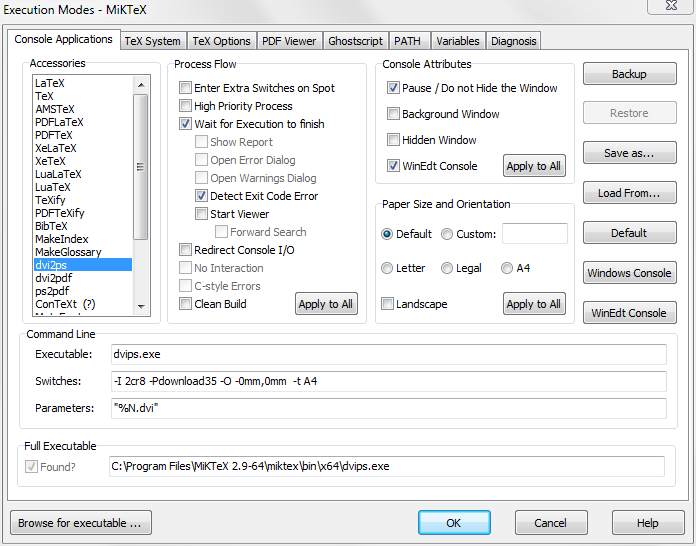
\includegraphics[bb=0 0 696 546,width=\textwidth]{eps/dvipsbmeps.png}}

\section{Enable JPG Images in DVIPS}

bm2eps also converts jpeg files, just use it as follows:

{\small
\verb"\centerline{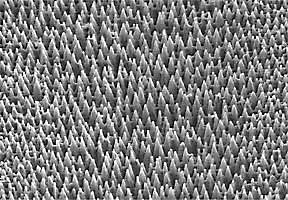
\includegraphics[bb= 0 0 288 200,width=0.5\textwidth ]{pic/light_trap2.jpg}}"
}


\centerline{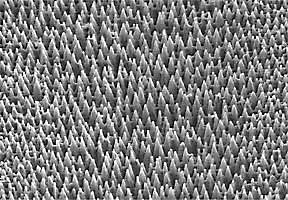
\includegraphics[bb= 0 0  288 200,width=0.5\textwidth]{pic/light_trap2.jpg}}




\section{Control Font Download to the PS File}

In the previous graph the dvi2ps application is also instructed to download the `standard Adobe' fonts to the PS file, by entering the option

\lstinline{ -Pdownload35}


\section{Setting up the Page Size for dvi2ps}

To set the page size in dvi2ps, add the following additional text to the dvi2ps switches:

\lstinline{-I 2cr8 -Pdownload35 -O -0mm,0mm  -t A4}


\section{Setting up the Page Size for ps2pdf}

Activate
$<$Options$>$$<$Execution Modes$>$ and select the ps2pdf entry in the 'Accessories' list box. Then change the page size as shown in the next figure. It does not make sense that the A4 should be in effect when the page size is set to default, but it does seem to work.

\centerline{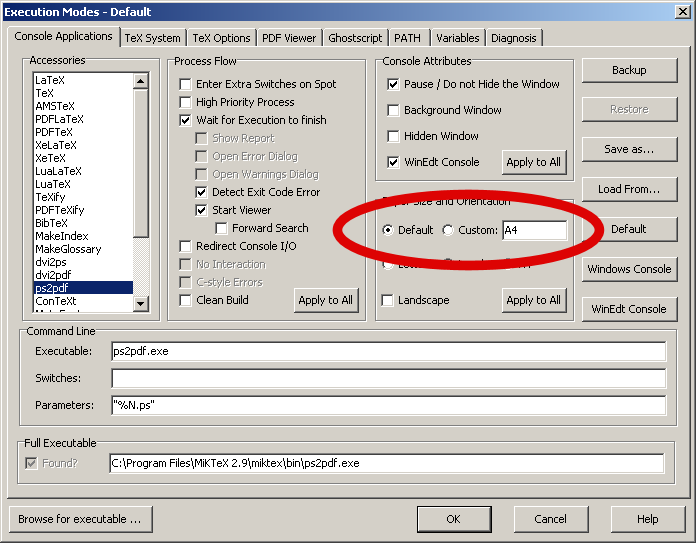
\includegraphics[bb= 0 0 696 543,width=\textwidth]{eps/ps2pdfpagesize.png}}

%Open the file \verb"C:\Program Files\WinEdt Team\WinEdt 10Exec\TeX\ps2pdf.edt"
%and do the following change
%
%\begin{verbatim}
%  //LetReg(4,'');
%  LetReg(4, "%!4 -sPAPERSIZE=a4");
%\end{verbatim}





\section{Enable File Update Warnings}

Sometimes you update a file externally (e.g. subversion updates the file version) and you want to be warned of this event.

$<$Options$>$$<$Options Interface$>$$<$Editor: Mouse, Modes.....$>$$<$Defaults$>$, edit the macro file just opened. Set the text shown below at the indicated location.

\centerline{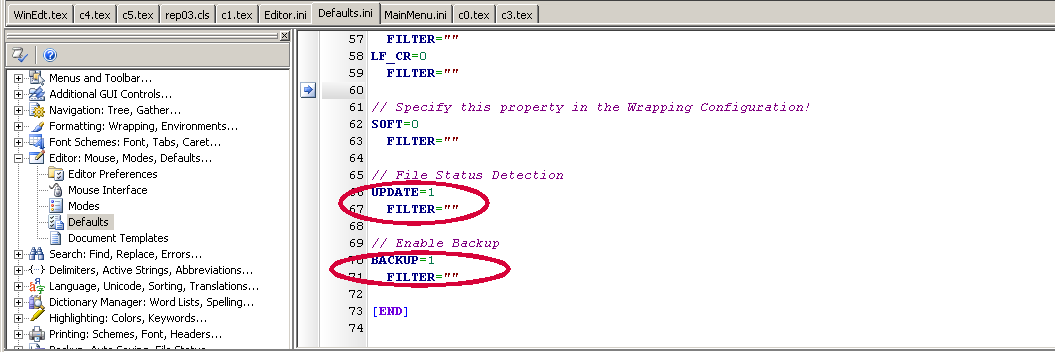
\includegraphics[bb= 0 0 1055 352,width=\textwidth]{eps/updatedrives.png}}




\section{Enable Multiple Instances of WinEdt}



$<$Options$>$$<$Options Interface$>$$<$Application: Projects, Forms, ....$>$$<$Additional Preferences$>$, near line 54 set the value.

Open an instance of WinEdt on the commandline with the following:

WinEdt -C="window title"


\section{Colour Theme}

To set a colour theme select from the 
$<$Options$>$$<$Theme$>$$<$ menu.  If this does not work, experiment with \\
$<$Options$>$$<$Options Interface$>$$<$Highlighting, Colors ...$>$$<$Colors$>$. Scroll to \lstinline{Solarized Light} and uncomment the theme you require, and comment out all those not required.  Now it is a bit of a hit-and-miss using the menu options and selecting \lstinline{Default} from an empty list, to get the scheme to work.


\section{See also}

\url{http://nakhmani.wordpress.com/2010/09/28/winedt-6-configuration/#more-44}


